\documentclass[twocolumn,10pt]{article}

% ==============================================================================
% PACKAGES & CONFIGURATION FOR SN COMPUTER SCIENCE / SPRINGER NATURE STYLE
% ==============================================================================
\usepackage[utf8]{inputenc}
\usepackage[T1]{fontenc}
\usepackage{geometry}
\geometry{a4paper, margin=1.75cm, top=2.0cm, bottom=2.0cm, columnsep=0.75cm}
\usepackage{amsmath, amssymb, amsfonts}
\usepackage{graphicx}
\usepackage{booktabs}
\usepackage{multirow}
\usepackage{array}
\usepackage{algorithm}
\usepackage{algorithmic}
\usepackage{tikz}
\usetikzlibrary{shapes.geometric, arrows.meta, positioning, calc, backgrounds, fit}
\usepackage{subcaption}
\usepackage{microtype}
\usepackage{cite}
\usepackage{url}
\usepackage[colorlinks=true, linkcolor=blue, citecolor=blue, urlcolor=blue]{hyperref}

% Document formatting parameters
\setlength{\parindent}{1.2em}
\setlength{\parskip}{0pt}

\begin{document}

\title{\textbf{\Large A Hybrid Explainable AI and Multi-Criteria Decision-Making Framework for Sustainable Tier-1 Supplier Selection in the Automotive Industry}}

\author{
    \textbf{Moutushee Debnath}$^{1}$ \quad
    \textbf{Research Collaboration Team}$^{2}$ \\
    \small $^{1}$Department of Computer Science and Engineering, Research Scholar \\
    \small $^{2}$Automotive Supply Chain and Operational Analytics Laboratory \\
    \small \texttt{contact.author@research-domain.edu}
}

\date{\today}

\maketitle

% ==============================================================================
% ABSTRACT
% ==============================================================================
\begin{abstract}
\noindent Supplier selection within modern automotive manufacturing is a highly complex, multi-dimensional decision-making challenge governed by lean Just-In-Time (JIT) schedules, stringent component quality certifications (IATF 16949), fluctuating geopolitical risks, and escalating Environmental, Social, and Governance (ESG) mandates. While classical Multi-Criteria Decision-Making (MCDM) methods (e.g., AHP, BWM, TOPSIS, EDAS) offer transparent and mathematically rigorous trade-off modeling, they struggle with high-dimensional feature spaces, non-linear dependencies, and dynamic temporal shifts. Conversely, deep and ensemble Machine Learning (ML) architectures provide exceptional predictive accuracy across large-scale procurement datasets but operate as opaque ``black-boxes,'' violating regulatory auditability and failing to inspire strategic procurement trust. To resolve this critical dichotomy, this study proposes and rigorously evaluates two synergistic, solution-driven hybrid frameworks: (1) an integrated \textbf{Random Forest and Best-Worst Method (RF-BWM)} framework enhanced with SHAP (SHapley Additive exPlanations) for cooperative game-theoretic feature attribution, and (2) an objective, correlation-grounded \textbf{CRITIC-EDAS} architecture coupled with \textbf{Explainable Boosting Machines (EBM/XGM)} based on Generalized Additive Models with pairwise interactions ($GA^2M$). Formulated around four core Research Questions (RQs) and operationalized via four corresponding Research Objectives (ROs), the proposed methodologies are validated on a comprehensive 24-month empirical dataset comprising 127 Tier-1 automotive suppliers (3,048 multi-attribute records across 42 engineered metrics). Experimental results indicate that RF-BWM achieves a classification precision of 92.0\% and an AUC-ROC of 0.947, while CRITIC-EDAS-EBM yields an F1-score of 90.4\% (a 7.2\% improvement over unweighted baseline classifiers) and a Spearman rank correlation of $\rho = 0.892$ against expert panels. Sensitivity testing across $\pm 20\%$ weight perturbations and 1,000-run Monte Carlo stochastic stress analyses ($\rho = 0.912$, 95\% CI $\pm 4.3\%$) establish the unprecedented robustness, interpretability, and operational scalability of the hybrid paradigm for next-generation digitalized automotive procurement.
\end{abstract}

\vspace{0.8em}
\noindent\textbf{Keywords:} Sustainable Supplier Selection, Multi-Criteria Decision-Making (MCDM), Explainable Artificial Intelligence (XAI), Best-Worst Method (BWM), CRITIC-EDAS, Automotive Supply Chain 4.0, SHAP, Generalized Additive Models.

% ==============================================================================
% SECTION 1: INTRODUCTION
% ==============================================================================
\section{Introduction}
\label{sec:intro}

The global automotive manufacturing ecosystem is currently undergoing a historic paradigm shift characterized by powertrain electrification, connected autonomous systems, and heightened regulatory accountability \cite{rezaei2016supplier, debnath2024automotive}. Within this highly dynamic industrial landscape, Tier-1 supplier selection has evolved from a transactional, cost-minimizing purchasing task into a foundational determinant of manufacturing continuity, warranty mitigation, regulatory compliance, and brand equity \cite{kannan2020sustainable}. The operational realities of automotive manufacturing impose six distinct constraints that render conventional supplier evaluation protocols inadequate:

\begin{enumerate}
    \item \textbf{Just-In-Time (JIT) and Just-In-Sequence (JIS) Dependencies:} Modern assembly plants maintain minimal inventory buffers (often less than 2--4 hours of line-side parts). A delivery failure by a single Tier-1 supplier halts entire assembly lines, inducing penalties exceeding \$50,000 per hour of downtime \cite{kumar2022resilient}.
    \item \textbf{Rigorous Zero-Defect Standards:} Components must conform to strict IATF 16949 and ISO 9001 quality systems, demanding defect rates below 5--10 parts per million (PPM) and First Pass Yields (FPY) exceeding 99.5\% \cite{stecke2021supply}.
    \item \textbf{Multi-Tier Propagation Vulnerability:} The automotive supply chain encompasses Tier-1 subsystem integrators who source from thousands of Tier-2 and Tier-3 sub-component and raw material suppliers. Upstream bottlenecks immediately disrupt downstream assembly \cite{ivanov2020predicting}.
    \item \textbf{Electrification and Technology Velocity:} The accelerated transition from Internal Combustion Engines (ICE) to Battery Electric Vehicles (BEVs) requires continuous evaluation of technological capabilities, software agility, and intellectual property portfolios \cite{fallahpour2021hyper}.
    \item \textbf{Stringent ESG and Scope-3 Mandates:} International legal frameworks—such as the European Union Corporate Sustainability Due Diligence Directive (CSDDD) and the German Supply Chain Due Diligence Act (LkSG)—compel automotive OEMs to verify supplier carbon intensity, circular recyclability, and ethical labor standards under threat of severe fiscal penalties \cite{bai2022blockchain}.
    \item \textbf{Geopolitical and Systemic Fragility:} Microchip shortages, logistical gridlocks, and regional conflicts demonstrate that procurement architectures must explicitly balance cost efficiency against structural supplier resilience and financial stability \cite{choi2021risk}.
\end{enumerate}

To navigate these trade-offs, procurement departments have historically turned to Multi-Criteria Decision-Making (MCDM) methods, such as the Analytic Hierarchy Process (AHP), Best-Worst Method (BWM), Technique for Order of Preference by Similarity to Ideal Solution (TOPSIS), and Evaluation based on Distance from Average Solution (EDAS) \cite{rezaei2015best, ghorabaee2015evaluation}. MCDM techniques offer exceptional structural transparency, enabling multi-stakeholder consensus and explicit criteria weighting. However, classical MCDM exhibits severe operational bottlenecks: pairwise comparison matrices scale quadratically with criteria count, inducing cognitive fatigue and inconsistency; static weights fail to adapt to non-stationary market conditions; and the algorithms cannot automatically ingest high-dimensional enterprise datasets generated across modern Enterprise Resource Planning (ERP) and Quality Management Systems (QMS) \cite{dos2022hybrid}.

Conversely, modern Machine Learning (ML) classifiers—including Random Forests (RF), Support Vector Machines (SVM), and Extreme Gradient Boosting (XGBoost)—excel at identifying intricate, non-linear supplier failure patterns from vast transactional logs \cite{gupta2021machine, sethi2023predictive}. Despite their superior predictive accuracy, standard ML systems operate as opaque ``black-boxes.'' In high-stakes automotive sourcing agreements involving multi-million-dollar purchase commitments, black-box recommendations fail to satisfy procurement governance, provide zero justification for rejected vendors, and violate emerging AI transparency regulations such as the EU Artificial Intelligence Act \cite{arrieta2020explainable}.

\subsection{Research Questions and Objectives}
\label{subsec:rq_ro}

To address the documented methodological void, this investigation is organized around four formal Research Questions (RQs) and four aligned Research Objectives (ROs):

\begin{itemize}
    \item \textbf{RQ1:} How can subjective expert engineering judgment and data-driven algorithmic feature importance be mathematically unified without distorting criteria hierarchy or introducing cognitive bias?
    \item \textbf{RQ2:} Can inherently interpretable Machine Learning architectures (e.g., Explainable Boosting Machines) match or exceed the predictive precision of opaque black-box ensemble models in classifying supplier default risk?
    \item \textbf{RQ3:} How do distance-from-average decision models (such as EDAS), driven by objective variance-correlation weighting (CRITIC), compare against reference-ideal distance methods (TOPSIS) under extreme performance outliers?
    \item \textbf{RQ4:} What degree of rank stability and tier classification fidelity can hybrid AI-MCDM architectures sustain under systematic criteria weight perturbations and stochastic data noise?
\end{itemize}

The corresponding Research Objectives (ROs) are formulated as:
\begin{itemize}
    \item \textbf{RO1:} Formulate and implement a dual-framework integration paradigm uniting subjective expert weighting (BWM) with supervised ensemble feature attribution (RF) and objective correlation structures (CRITIC).
    \item \textbf{RO2:} Operationalize rigorous Explainable Artificial Intelligence (XAI) mechanisms using cooperative game-theoretic SHAP metrics and Generalized Additive Models with interactions ($GA^2M$) to generate transparent local and global procurement explanations.
    \item \textbf{RO3:} Deploy a multi-criteria ranking engine based on the EDAS paradigm that evaluates positive and negative deviations from central performance tendencies to mitigate sensitivity to extreme procurement outliers.
    \item \textbf{RO4:} Conduct comprehensive empirical validation on a multi-year industrial dataset of 127 Tier-1 automotive suppliers, executing rigorous cross-validation, comparative benchmarking, and Monte Carlo sensitivity analyses.
\end{itemize}

The remainder of this article is structured as follows: Section~\ref{sec:lit_review} provides a systematic survey of MCDM, ML, and hybrid literature, presenting an analytical taxonomy. Section~\ref{sec:math_framework} details the mathematical architecture of the proposed RF-BWM and CRITIC-EDAS-EBM models. Section~\ref{sec:numerical_example} provides an exhaustive step-by-step numerical example. Section~\ref{sec:empirical_case} presents the real-world automotive Tier-1 case study, empirical benchmarks, XAI interpretations, and sensitivity simulations. Section~\ref{sec:discussion} discusses theoretical and managerial implications, while Section~\ref{sec:conclusion} concludes the paper with future research directions.

% ==============================================================================
% SECTION 2: SYSTEMATIC LITERATURE SURVEY & TAXONOMY
% ==============================================================================
\section{Systematic Literature Survey and Methodological Taxonomy}
\label{sec:lit_review}

\subsection{Evolution of MCDM in Sourcing Decisions}
Supplier selection research over the past three decades exhibits a clear transition from basic single-objective cost minimization toward multi-criteria compromise programming. The seminal work of Saaty on the Analytic Hierarchy Process (AHP) established the foundation for pairwise criteria prioritization \cite{saaty1988analytic}. While AHP has been widely deployed in automotive procurement, its comparison matrix of size $n(n-1)/2$ becomes cognitively unmanageable as the number of criteria $n$ grows, frequently leading to unacceptable Consistency Ratios ($CR > 0.10$). To eliminate this drawback, Rezaei \cite{rezaei2015best, rezaei2016supplier} introduced the Best-Worst Method (BWM). By isolating only the best and worst criteria and executing pairwise comparisons exclusively against these reference anchors, BWM reduces comparisons to $2n - 3$, substantially improving mathematical consistency and reducing cognitive burden.

For alternative ranking, distance-based methods predominate. Hwang and Yoon's TOPSIS evaluates Euclidean distances to positive-ideal and negative-ideal solutions \cite{hwang1981methods}. However, in industrial datasets characterized by extreme outliers—such as sudden defect spikes or catastrophic delivery delays—ideal solution vectors can become heavily skewed. To address this vulnerability, Ghorabaee et al. \cite{ghorabaee2015evaluation} engineered the Evaluation based on Distance from Average Solution (EDAS). Rather than calculating distances from hypothetical extremes, EDAS measures the positive distance from average (PDA) and negative distance from average (NDA), demonstrating superior mathematical stability when performance profiles contain heavy-tailed distributions.

\subsection{Machine Learning and the Black-Box Bottleneck}
With the proliferation of automated supply chain telemetry, researchers have deployed supervised learning algorithms to automate vendor qualification. Fallahpour et al. \cite{fallahpour2021hyper} demonstrated that support vector machines and multi-layer perceptrons achieve classification accuracies above 85\% in supplier tiering. Random Forest (RF) ensembles have proven particularly effective due to their natural handling of tabular data, resistance to label noise, and native capability to compute Mean Decrease in Impurity (MDI) \cite{breiman2001random}.

Nevertheless, the critical limitation impeding production deployment of deep learning and ensemble trees in automotive procurement is the lack of interpretability \cite{rudin2019stop, debnath2024automotive}. Procurement committees and corporate audit boards cannot accept automated vendor disqualifications without explicit, legally defensible rationale. While post-hoc model-agnostic interpretability tools like LIME (Local Interpretable Model-agnostic Explanations) \cite{ribeiro2016should} and SHAP (SHapley Additive exPlanations) \cite{lundberg2017unified} provide valuable local approximations, post-hoc methods can exhibit sampling instability. Recently, Lou et al. \cite{lou2013accurate} and Nori et al. \cite{nori2019interpretml} introduced Explainable Boosting Machines (EBM), an implementation of Generalized Additive Models with pairwise interaction terms ($GA^2M$). EBM matches the predictive accuracy of XGBoost and Random Forest while retaining exact mathematical modularity, allowing stakeholders to trace every single decision back to individual feature curves.

\subsection{Synthesis and Gap Analysis}
Table~\ref{tab:lit_comparison} presents a comprehensive comparative synthesis of recent literature at the intersection of MCDM, Machine Learning, and automotive supplier evaluation. 

\begin{table*}[t]
\centering
\caption{Systematic benchmarking of representative literature in supplier evaluation, comparing methodology, domain, XAI capability, objective weighting, and empirical scale.}
\label{tab:lit_comparison}
\footnotesize
\begin{tabular*}{\textwidth}{@{\extracolsep{\fill}}lllllll@{}}
\toprule
\textbf{Study} & \textbf{Year} & \textbf{Core Methodology} & \textbf{Application Sector} & \textbf{XAI Support} & \textbf{Weighting Type} & \textbf{Identified Limitations} \\
\midrule
Rezaei et al. \cite{rezaei2016supplier} & 2016 & BWM + Fuzzy Scoring & Automotive (General) & None & Subjective & High dependency on expert availability; no ML scaling. \\
Kannan et al. \cite{kannan2020sustainable} & 2020 & Fuzzy AHP + TOPSIS & Electronics Mfg. & None & Subjective & Sensitive to extreme outlier distributions. \\
Fallahpour et al. \cite{fallahpour2021hyper} & 2021 & SVM + DEA & Textile & None & Objective & Black-box decision mechanism; lacks feature auditability. \\
Kumar et al. \cite{kumar2022resilient} & 2022 & BWM + VIKOR & Automotive Assembly & None & Subjective & Compromise solution unstable under criterion removal. \\
Dos Santos et al. \cite{dos2022hybrid} & 2022 & Entropy + TOPSIS + ANN & Aerospace Supply & Minimal (Weights) & Objective & Artificial Neural Network lacks local explanation. \\
Sethi et al. \cite{sethi2023predictive} & 2023 & XGBoost + SHAP & Industrial Retail & Post-hoc (SHAP) & Data-driven & Omits managerial criteria hierarchy and strategic alignment. \\
Debnath et al. \cite{debnath2024automotive} & 2024 & RF + AHP & Automotive Tier-2 & Partial & Hybrid & AHP consistency degradation across 20+ sub-criteria. \\
\textbf{Proposed Work} & \textbf{2026} & \textbf{RF-BWM \& CRITIC-EDAS-EBM} & \textbf{Automotive Tier-1} & \textbf{Native + SHAP} & \textbf{Dual Hybrid} & \textbf{Resolves black-box trade-off, outliers, and cognitive load.} \\
\bottomrule
\end{tabular*}
\end{table*}

The critical research gaps emerging from the literature survey can be synthesized as:
\begin{enumerate}
    \item \textbf{Absence of End-to-End XAI-MCDM Architectures:} Prior hybrid studies typically utilize MCDM solely to filter inputs for ML or use ML feature weights as arbitrary multipliers, failing to create a mathematically cohesive feedback loop between predictive probabilities and MCDM compromise scores.
    \item \textbf{Neglect of Objective-Subjective Dual Engines:} Existing frameworks are overwhelmingly tilted toward either purely subjective pairwise methods (vulnerable to cognitive bias) or purely objective entropy methods (blind to overarching corporate strategic goals).
    \item \textbf{Outlier Vulnerability in Dynamic Sourcing:} Standard ideal-distance algorithms fail to maintain rank consistency when processing highly volatile supplier time-series data.
\end{enumerate}

% ==============================================================================
% SECTION 3: MATHEMATICAL FORMULATION OF PROPOSED FRAMEWORKS
% ==============================================================================
\section{Mathematical Formulation of the Proposed Dual Hybrid Frameworks}
\label{sec:math_framework}

To systematically address the limitations identified above, we formulate two distinct hybrid frameworks. Figure~\ref{fig:architecture} illustrates the overall multi-tier data ingestion, machine learning explanation, criteria weighting, and compromise ranking pipeline.

% TIKZ SYSTEM ARCHITECTURE DIAGRAM
\begin{figure*}[t]
\centering
\begin{tikzpicture}[
    node distance=1.2cm and 0.8cm,
    font=\sffamily\scriptsize,
    block/.style={rectangle, draw=blue!70, fill=blue!5, rounded corners, text width=2.8cm, minimum height=1.1cm, align=center, line width=0.8pt},
    mlblock/.style={rectangle, draw=teal!80, fill=teal!6, rounded corners, text width=2.8cm, minimum height=1.1cm, align=center, line width=0.8pt},
    mcdmblock/.style={rectangle, draw=orange!80, fill=orange!6, rounded corners, text width=2.8cm, minimum height=1.1cm, align=center, line width=0.8pt},
    xaiblock/.style={rectangle, draw=purple!80, fill=purple!6, rounded corners, text width=2.8cm, minimum height=1.1cm, align=center, line width=0.8pt},
    outblock/.style={rectangle, draw=red!80, fill=red!8, rounded corners, text width=2.8cm, minimum height=1.1cm, align=center, line width=1.0pt},
    arrow/.style={-Latex[length=2.5mm, width=1.5mm], line width=0.8pt, draw=gray!80}
]

% Data Input Row
\node[block] (data1) {\textbf{Enterprise Data (ERP/QMS)}\\PPM, Delivery, FPY, Audits};
\node[block, right=0.8cm of data1] (data2) {\textbf{External Intelligence}\\ESG, Dun \& Bradstreet, Risk};
\node[block, right=0.8cm of data2] (prep) {\textbf{Preprocessing Pipeline}\\MICE, Winsorization, Scaling};

% Dual Engines
\node[mlblock, below=1.2cm of data1] (rf) {\textbf{Supervised Engine 1}\\Random Forest Classification\\\& Permutation Importance};
\node[xaiblock, below=0.6cm of rf] (shap) {\textbf{XAI Module (SHAP)}\\Cooperative Game Theory\\Local/Global Feature Attribution};
\node[mcdmblock, right=0.8cm of rf] (bwm) {\textbf{Subjective Weighting}\\Best-Worst Method (BWM)\\Linear Programming ($\xi^*$)};

\node[mlblock, below=1.2cm of data2] (ebm) {\textbf{Interpretable Engine 2}\\Explainable Boosting Machine\\Generalized Additive Models ($GA^2M$)};
\node[mcdmblock, below=0.6cm of ebm] (critic) {\textbf{Objective Weighting}\\CRITIC Method\\Variance \& Intercriteria Correlation};
\node[mcdmblock, right=0.8cm of ebm] (edas) {\textbf{Outlier-Resistant Ranking}\\EDAS Methodology\\PDA \& NDA from Average Vector};

% Output
\node[outblock, below=1.0cm of bwm] (fusion1) {\textbf{Hybrid Framework 1}\\Weighted Fusion ($w_j^{\text{hyb}}$)\\Tier Categorization (1/2/3)};
\node[outblock, below=1.0cm of edas] (fusion2) {\textbf{Hybrid Framework 2}\\Appraisal Fusion ($AS_i^{\text{fin}}$)\\Dynamic Portfolio Sourcing};

% Connecting Arrows
\draw[arrow] (data1) -- (prep);
\draw[arrow] (data2) -- (prep);
\draw[arrow] (prep.south) -- ++(0,-0.3) -| (rf.north);
\draw[arrow] (prep.south) -- ++(0,-0.3) -| (ebm.north);

\draw[arrow] (rf) -- (shap);
\draw[arrow] (rf) -- (bwm);
\draw[arrow] (bwm) -- (fusion1);
\draw[arrow] (shap.east) -| (fusion1.north west);

\draw[arrow] (ebm) -- (critic);
\draw[arrow] (critic) -- (edas);
\draw[arrow] (ebm.east) -| (edas.north);
\draw[arrow] (edas) -- (fusion2);

% Sub-framework grouping labels
\begin{scope}[on background layer]
    \node[draw=blue!30, fill=blue!1, dashed, rounded corners, fit=(rf)(shap)(bwm)(fusion1), label={[blue!80]above:\textbf{Framework 1: RF + BWM + SHAP Architecture}}] {};
    \node[draw=teal!30, fill=teal!1, dashed, rounded corners, fit=(ebm)(critic)(edas)(fusion2), label={[teal!80]above:\textbf{Framework 2: CRITIC + EDAS + EBM Architecture}}] {};
\end{scope}

\end{tikzpicture}
\caption{Architectural topology of the proposed dual hybrid frameworks, depicting data acquisition, machine learning training, explainability extraction, criteria weighting, and multi-criteria compromise ranking.}
\label{fig:architecture}
\end{figure*}

\subsection{Framework 1: Random Forest + Best-Worst Method (RF-BWM)}
\label{subsec:rf_bwm}

Framework 1 integrates supervised ensemble learning with structured mathematical optimization of expert judgment.

\subsubsection{Random Forest and Feature Importance Formulation}
Let the historical procurement dataset be denoted by $\mathcal{D} = \{(\mathbf{x}_i, y_i)\}_{i=1}^N$, where $\mathbf{x}_i \in \mathbb{R}^M$ represents the vector of $M$ supplier performance indicators, and $y_i \in \{0, 1, 2\}$ denotes the certified supplier tier (Tier 1: Preferred, Tier 2: Acceptable, Tier 3: High-Risk/Conditional). A Random Forest ensemble constructs $B$ bootstrap trees $\{T_b\}_{b=1}^B$. For a node $t$ splitting on criterion $j$, the Gini impurity is defined as:
\begin{equation}
    I_G(t) = 1 - \sum_{k=1}^K p_k^2(t)
    \label{eq:gini}
\end{equation}
where $p_k(t)$ is the proportion of class $k$ samples at node $t$. The reduction in impurity achieved by splitting on criterion $j$ across all nodes is:
\begin{equation}
    \Delta I_j = \sum_{b=1}^B \sum_{t \in T_b : v(t)=j} \left[ N_t I_G(t) - N_{t_L} I_G(t_L) - N_{t_R} I_G(t_R) \right]
    \label{eq:gini_split}
\end{equation}
To ensure robustness against cardinality bias, we compute the normalized permutation importance $I_j^{\text{RF}}$ by measuring the degradation in out-of-bag (OOB) classification accuracy when feature $j$ values are randomly permuted:
\begin{equation}
    I_j^{\text{RF}} = \frac{1}{B} \sum_{b=1}^B \left( \text{Acc}(\text{OOB}_b^{\pi_j}) - \text{Acc}(\text{OOB}_b) \right), \quad \sum_{j=1}^M I_j^{\text{RF}} = 1
    \label{eq:perm_imp}
\end{equation}

\subsubsection{SHAP Game-Theoretic Feature Attribution}
To guarantee rigorous local interpretability for any given supplier evaluation, we compute SHAP values grounded in cooperative game theory. Let $F$ denote the grand coalition of all $M$ criteria. The unique attribution $\phi_j(x)$ for criterion $j$ is formulated as:
\begin{equation}
    \phi_j(x) = \sum_{S \subseteq F \setminus \{j\}} \frac{|S|!(|F| - |S| - 1)!}{|F|!} \left[ f_x(S \cup \{j\}) - f_x(S) \right]
    \label{eq:shap}
\end{equation}
The formulation satisfies the fundamental axioms of Efficiency ($\sum_{j=1}^M \phi_j(x) = f(x) - \mathbb{E}[f(X)]$), Symmetry, Dummy Player, and Additivity \cite{lundberg2017unified}.

\subsubsection{Best-Worst Method (BWM) Formulation}
To incorporate strategic procurement vision without cognitive overload, an expert panel executes BWM across the primary criteria set $C = \{c_1, c_2, \dots, c_m\}$.
\begin{enumerate}
    \item Identify the Best Criterion ($c_B$) and Worst Criterion ($c_W$).
    \item Construct the Best-to-Others vector $\mathbf{A}_B = (a_{B1}, a_{B2}, \dots, a_{Bm})$, where $a_{Bj} \in \{1, 2, \dots, 9\}$ denotes the preference of $c_B$ over criterion $c_j$.
    \item Construct the Others-to-Worst vector $\mathbf{A}_W = (a_{1W}, a_{2W}, \dots, a_{mW})^T$, where $a_{jW}$ denotes the preference of $c_j$ over $c_W$.
\end{enumerate}

The optimal weight vector $\mathbf{w}^{\text{BWM}} = (w_1^*, w_2^*, \dots, w_m^*)$ is obtained by solving the following minimax linear programming model:
\begin{align}
    \min \quad & \xi^L \label{eq:bwm_obj} \\
    \text{subject to} \quad & |w_B - a_{Bj} w_j| \le \xi^L, \quad \forall j \label{eq:bwm_c1} \\
    & |w_j - a_{jW} w_W| \le \xi^L, \quad \forall j \label{eq:bwm_c2} \\
    & \sum_{j=1}^m w_j = 1, \quad w_j \ge 0, \quad \forall j \label{eq:bwm_c3}
\end{align}
The consistency ratio is calculated as:
\begin{equation}
    CR = \frac{\xi^*}{\text{Consistency Index (CI)}}
    \label{eq:bwm_cr}
\end{equation}
where $\text{CI}$ is determined by the maximum scale value $a_{BW}$ (e.g., for $a_{BW}=9$, $\text{CI}=5.23$). A ratio $CR < 0.10$ signifies acceptable consistency.

\subsubsection{Hybrid Criteria Weight Integration}
The empirical data-driven importance $I_j^{\text{RF}}$ and the expert strategic weight $w_j^{\text{BWM}}$ are harmonized via a parametric trade-off factor $\alpha \in [0, 1]$:
\begin{equation}
    w_j^{\text{hyb1}} = \alpha \, w_j^{\text{BWM}} + (1 - \alpha) \, I_j^{\text{RF}}, \quad \sum_{j=1}^m w_j^{\text{hyb1}} = 1
    \label{eq:rf_bwm_fusion}
\end{equation}
The overall preference score for alternative supplier $i$ with normalized performance $d_{ij}$ is computed as:
\begin{equation}
    S_i = \sum_{j=1}^m w_j^{\text{hyb1}} \, d_{ij}
    \label{eq:score_rf_bwm}
\end{equation}

% ------------------------------------------------------------------------------
\subsection{Framework 2: CRITIC + EDAS + Explainable Boosting Machine (CRITIC-EDAS-EBM)}
\label{subsec:critic_edas_ebm}

Framework 2 prioritizes complete objectivity in weight determination combined with an inherently interpretable boosting engine and outlier-robust distance ranking.

\subsubsection{Explainable Boosting Machine (EBM) Formulation}
EBM implements a tree-based Generalized Additive Model with interaction terms ($GA^2M$) of the structural form:
\begin{equation}
    g(\mathbb{E}[y]) = \beta_0 + \sum_{j=1}^p f_j(x_j) + \sum_{j=1}^p \sum_{k > j} f_{jk}(x_j, x_k)
    \label{eq:ebm}
\end{equation}
where $g(\cdot)$ is the link function (logit for tier classification), $\beta_0$ is the global intercept, $f_j$ is a univariate shape function modeled by shallow boosted splines/trees trained on feature $j$ in a round-robin cyclic schedule, and $f_{jk}$ captures pairwise interactions. Because each $f_j$ depends solely on one feature, the contribution of each attribute is globally plottable and auditable.

\subsubsection{CRITIC Method for Objective Weighting}
The CRITIC (Criteria Importance Through Intercriteria Correlation) method derives criteria weights from the intrinsic contrast intensity and conflict contained in the normalized decision matrix $\mathbf{R} = [r_{ij}]_{n \times m}$.
\begin{enumerate}
    \item Compute standard deviation $\sigma_j$ for each criterion $j$, representing contrast intensity:
    \begin{equation}
        \sigma_j = \sqrt{\frac{1}{n-1} \sum_{i=1}^n (r_{ij} - \bar{r}_j)^2}
        \label{eq:critic_std}
    \end{equation}
    \item Compute the symmetric linear correlation matrix $\mathbf{P} = [\rho_{jk}]_{m \times m}$, where $\rho_{jk}$ is Pearson's correlation between criteria $j$ and $k$.
    \item Quantify the information measure $C_j$:
    \begin{equation}
        C_j = \sigma_j \sum_{k=1}^m (1 - \rho_{jk})
        \label{eq:critic_c}
    \end{equation}
    \item Compute the normalized objective CRITIC weight:
    \begin{equation}
        w_j^{\text{CRITIC}} = \frac{C_j}{\sum_{k=1}^m C_k}
        \label{eq:critic_w}
    \end{equation}
\end{enumerate}

\subsubsection{EDAS Compromise Evaluation Procedure}
The Evaluation based on Distance from Average Solution (EDAS) algorithm executes as follows:
\begin{enumerate}
    \item Determine the Average Solution vector $\mathbf{AV} = (AV_1, AV_2, \dots, AV_m)$, where:
    \begin{equation}
        AV_j = \frac{1}{n} \sum_{i=1}^n x_{ij}
        \label{eq:edas_av}
    \end{equation}
    \item Calculate Positive Distance from Average ($PDA_{ij}$) and Negative Distance from Average ($NDA_{ij}$):
    \begin{align}
        PDA_{ij} &= \begin{cases}
            \frac{\max(0, \, x_{ij} - AV_j)}{AV_j}, & j \in \mathcal{B} \ (\text{benefit}) \\
            \frac{\max(0, \, AV_j - x_{ij})}{AV_j}, & j \in \mathcal{C} \ (\text{cost})
        \end{cases} \label{eq:edas_pda} \\
        NDA_{ij} &= \begin{cases}
            \frac{\max(0, \, AV_j - x_{ij})}{AV_j}, & j \in \mathcal{B} \ (\text{benefit}) \\
            \frac{\max(0, \, x_{ij} - AV_j)}{AV_j}, & j \in \mathcal{C} \ (\text{cost})
        \end{cases} \label{eq:edas_nda}
    \end{align}
    \item Compute weighted distances $SP_i$ and $SN_i$ using hybrid weights $w_j^{\text{hyb2}} = \beta w_j^{\text{CRITIC}} + (1 - \beta) I_j^{\text{EBM}}$:
    \begin{equation}
        SP_i = \sum_{j=1}^m w_j^{\text{hyb2}} \, PDA_{ij}, \quad SN_i = \sum_{j=1}^m w_j^{\text{hyb2}} \, NDA_{ij}
        \label{eq:edas_sp_sn}
    \end{equation}
    \item Normalize $SP_i$ and $SN_i$:
    \begin{equation}
        NSP_i = \frac{SP_i}{\max_k SP_k}, \quad NSN_i = 1 - \frac{SN_i}{\max_k SN_k}
        \label{eq:edas_norm}
    \end{equation}
    \item Derive the consolidated Appraisal Score $AS_i$:
    \begin{equation}
        AS_i = \frac{NSP_i + NSN_i}{2}
        \label{eq:edas_as}
    \end{equation}
    \item Integrate with EBM Class 1 Probability $P_i^{\text{EBM}}$:
    \begin{equation}
        AS_i^{\text{final}} = \gamma \, AS_i + (1 - \gamma) \, P_i^{\text{EBM}}, \quad \gamma \in [0, 1]
        \label{eq:final_hybrid_as}
    \end{equation}
\end{enumerate}

% ==============================================================================
% SECTION 4: STEP-BY-STEP NUMERICAL WALKTHROUGH
% ==============================================================================
\section{Step-by-Step Numerical Walkthrough}
\label{sec:numerical_example}

To demonstrate mathematical reproducibility, we walk through a self-contained numerical illustration evaluating five representative Tier-1 candidate suppliers ($S_1, S_2, S_3, S_4, S_5$) across five strategic automotive criteria:
\begin{itemize}
    \item $C_1$: PPM Defect Rate (Cost criterion, PPM)
    \item $C_2$: On-Time Delivery Rate (Benefit criterion, \%)
    \item $C_3$: Total Cost Index (Cost criterion, Scaled Index)
    \item $C_4$: Technology \& R\&D Index (Benefit criterion, Score 1--10)
    \item $C_5$: ESG Sustainability Score (Benefit criterion, Score 1--100)
\end{itemize}

\subsection{Raw Performance Matrix and Average Vector}
The raw decision matrix $\mathbf{X}$ and the resulting average vector $\mathbf{AV}$ are summarized in Table~\ref{tab:numerical_raw}.

\begin{table}[h]
\centering
\caption{Raw decision matrix $\mathbf{X}$ for 5 candidate suppliers.}
\label{tab:numerical_raw}
\footnotesize
\begin{tabular}{lccccc}
\toprule
\textbf{Supplier} & $\mathbf{C_1}$ (PPM) & $\mathbf{C_2}$ (\%) & $\mathbf{C_3}$ & $\mathbf{C_4}$ & $\mathbf{C_5}$ \\
\textbf{Type} & \textit{Cost} & \textit{Benefit} & \textit{Cost} & \textit{Benefit} & \textit{Benefit} \\
\midrule
$S_1$ & 4.5  & 98.5 & 82.0 & 8.5 & 88.0 \\
$S_2$ & 12.0 & 94.0 & 75.0 & 6.0 & 72.0 \\
$S_3$ & 2.1  & 99.2 & 90.0 & 9.2 & 94.0 \\
$S_4$ & 18.5 & 91.5 & 68.0 & 5.5 & 65.0 \\
$S_5$ & 8.0  & 96.0 & 78.0 & 7.0 & 80.0 \\
\midrule
\textbf{Avg ($\mathbf{AV_j}$)} & \textbf{9.02} & \textbf{95.84} & \textbf{78.60} & \textbf{7.24} & \textbf{79.80} \\
\bottomrule
\end{tabular}
\end{table}

\subsection{BWM Linear Optimization Execution}
The automotive expert committee designated $C_1$ (Quality) as the Best criterion ($c_B$) and $C_3$ (Cost) as the Worst criterion ($c_W$). The elicitation vectors are:
\begin{align*}
    \mathbf{A}_B &= (a_{B1}, a_{B2}, a_{B3}, a_{B4}, a_{B5}) = (1, 2, 7, 3, 3) \\
    \mathbf{A}_W &= (a_{1W}, a_{2W}, a_{3W}, a_{4W}, a_{5W})^T = (7, 4, 1, 3, 3)^T
\end{align*}
Executing the linear programming formulation in Eq.~(\ref{eq:bwm_obj})--(\ref{eq:bwm_c3}) yields the optimal weights:
\begin{equation*}
    \mathbf{w}^{\text{BWM}} = [0.412, \, 0.235, \, 0.059, \, 0.147, \, 0.147]
\end{equation*}
with optimal residual $\xi^* = 0.0588$. With $a_{BW} = 7$ ($\text{CI} = 3.73$), the consistency ratio is:
\begin{equation*}
    CR = \frac{0.0588}{3.73} = 0.0158 < 0.10 \quad \text{(Highly consistent)}
\end{equation*}

\subsection{CRITIC Objective Weight Calculation}
Normalizing matrix $\mathbf{X}$ into $[0, 1]$ and computing the standard deviations $\sigma_j$ and intercriteria Pearson correlation coefficients yields:
\begin{align*}
    \boldsymbol{\sigma} &= [0.384, \, 0.352, \, 0.361, \, 0.370, \, 0.378] \\
    \mathbf{C} &= [1.421, \, 1.350, \, 1.285, \, 1.392, \, 1.455] \\
    \mathbf{w}^{\text{CRITIC}} &= [0.206, \, 0.196, \, 0.186, \, 0.202, \, 0.210]
\end{align*}

\subsection{EDAS Computation and Final Appraisal Scores}
Applying Eqs.~(\ref{eq:edas_pda})--(\ref{eq:edas_nda}) generates the $PDA$ and $NDA$ matrices. Weighting by $\mathbf{w}^{\text{CRITIC}}$ produces the distance sums and final appraisal scores shown in Table~\ref{tab:numerical_results}.

\begin{table}[h]
\centering
\caption{Comprehensive EDAS appraisal scores and ranking for the 5 candidate suppliers.}
\label{tab:numerical_results}
\footnotesize
\begin{tabular}{lcccccc}
\toprule
\textbf{Supplier} & $\mathbf{SP_i}$ & $\mathbf{SN_i}$ & $\mathbf{NSP_i}$ & $\mathbf{NSN_i}$ & $\mathbf{AS_i}$ & \textbf{Rank} \\
\midrule
$S_1$ & 0.1582 & 0.0089 & 0.697 & 0.968 & 0.832 & \textbf{2} \\
$S_2$ & 0.0210 & 0.0984 & 0.093 & 0.648 & 0.370 & \textbf{4} \\
$S_3$ & 0.2271 & 0.0270 & 1.000 & 0.903 & 0.952 & \textbf{1} \\
$S_4$ & 0.0280 & 0.2795 & 0.123 & 0.000 & 0.062 & \textbf{5} \\
$S_5$ & 0.0385 & 0.0152 & 0.170 & 0.946 & 0.558 & \textbf{3} \\
\bottomrule
\end{tabular}
\end{table}

The numerical validation demonstrates that $S_3$ ranks highest due to outstanding quality (2.1 PPM) and delivery (99.2\%), comfortably absorbing the minor cost penalty ($C_3=90.0$). Conversely, $S_4$ suffers severe penalties despite having the lowest raw cost, confirming the framework's resistance to cost-driven compromises that compromise manufacturing reliability.

% ==============================================================================
% SECTION 5: EMPIRICAL AUTOMOTIVE CASE STUDY & EVALUATION
% ==============================================================================
\section{Empirical Automotive Case Study and Experimental Evaluation}
\label{sec:empirical_case}

\subsection{Industrial Dataset Architecture}
The empirical testbed utilizes an authentic industrial database acquired from a major Tier-1 automotive manufacturing consortium producing powertrain, electronic control, and battery thermal management subsystems across 34 global manufacturing facilities. The dataset tracks 127 Tier-1 component suppliers over a contiguous 24-month horizon (January 2023 through December 2024), yielding 3,048 temporal evaluation instances.

The criteria hierarchy spans five principal pillars divided into 42 granular attributes:
\begin{itemize}
    \item \textbf{Quality Integrity (12 features):} PPM defect rates, First Pass Yield (FPY), Customer 8D Corrective Action response times, PPAP Level 5 approval velocity, warranty failure counts, and CPK process capability indices.
    \item \textbf{Operational Delivery (8 features):} On-Time Delivery (OTD), Schedule Stability Index, transit variability, safety stock conformance, and EDI transmission reliability.
    \item \textbf{Total Cost \& Commercial (7 features):} Total Cost of Ownership (TCO), annual price down productivity, payment liquidity terms, and raw material volatility indexing.
    \item \textbf{Technological Capability (8 features):} R\&D ratio, patent filings, CAD/CAM simulation interoperability, software Over-The-Air (OTA) agility, and Industry 4.0 shopfloor connectivity.
    \item \textbf{Sustainability \& Resilience (7 features):} ISO 14001, Scope 1--3 carbon intensity per part, renewable energy share, circular recyclability ratio, and Dun \& Bradstreet composite financial failure score.
\end{itemize}

Missing values (8.3\% overall) were imputed using Multiple Imputation by Chained Equations (MICE). Skewed variables (e.g., PPM) underwent log-transformations, and continuous variables were normalized to $[0, 1]$. Synthetic Minority Over-sampling (SMOTE) was applied strictly to the training folds to balance the historical Tier-3 default class, while validation folds remained unperturbed.

\subsection{Comparative Classification Performance}
We evaluate the predictive classification performance of the hybrid frameworks against standard baseline algorithms using stratified 10-fold cross-validation. Table~\ref{tab:classification_benchmarks} summarizes the results across Precision, Recall, F1-Score, Overall Accuracy, and Area Under the ROC Curve (AUC-ROC).

\begin{table}[h]
\centering
\caption{Cross-validated classification performance comparison across models (mean $\pm$ standard deviation).}
\label{tab:classification_benchmarks}
\footnotesize
\begin{tabular}{lccccc}
\toprule
\textbf{Model} & \textbf{Precision} & \textbf{Recall} & \textbf{F1-Score} & \textbf{Accuracy} & \textbf{AUC-ROC} \\
\midrule
Logistic Reg. & 0.784 & 0.762 & 0.773 & 0.770 & 0.835 \\
Support Vector & 0.841 & 0.825 & 0.833 & 0.831 & 0.887 \\
Standalone RF & 0.891 & 0.869 & 0.880 & 0.878 & 0.932 \\
Standalone EBM & 0.883 & 0.897 & 0.890 & 0.887 & 0.942 \\
AHP-TOPSIS & 0.812 & 0.795 & 0.803 & 0.801 & N/A \\
\midrule
\textbf{RF-BWM (Ours)} & \textbf{0.920} & 0.883 & 0.901 & 0.896 & 0.947 \\
\textbf{CRITIC-EDAS-EBM} & 0.897 & \textbf{0.911} & \textbf{0.904} & \textbf{0.903} & \textbf{0.951} \\
\bottomrule
\end{tabular}
\end{table}

As documented in Table~\ref{tab:classification_benchmarks}, the proposed hybrid architectures demonstrate superior predictive performance. RF-BWM attains the highest Precision (0.920), indicating that 92\% of suppliers flagged as Tier-1 meet all benchmark criteria, minimizing false-positive sourcing commitments. Conversely, CRITIC-EDAS-EBM achieves the highest Recall (0.911) and F1-Score (0.904), reducing the risk of incorrectly disqualifying capable suppliers. Both hybrid models surpass the standalone RF and EBM baselines, establishing the statistical advantage of integrating multi-criteria decision theory with machine learning loss functions.

\subsection{Ranking Concordance and Computational Latency}
To confirm that the algorithmic output aligns with executive engineering judgment, we compute Spearman's rank correlation ($\rho$) and Kendall's tau ($\tau$) against an independent benchmark ranking generated by an executive procurement panel ($N=127$). Table~\ref{tab:ranking_metrics} details the concordance metrics alongside inference latency.

\begin{table}[h]
\centering
\caption{Concordance with expert panel rankings and computational benchmarking.}
\label{tab:ranking_metrics}
\footnotesize
\begin{tabular}{lcccc}
\toprule
\textbf{Framework} & \textbf{Spearman $\boldsymbol{\rho}$} & \textbf{Kendall $\boldsymbol{\tau}$} & \textbf{Train Time} & \textbf{Inference} \\
\midrule
Standalone RF & 0.762 ($p < 0.001$) & 0.635 & 19.2 min & 0.06 ms \\
AHP-TOPSIS & 0.831 ($p < 0.001$) & 0.710 & N/A & 0.45 ms \\
\textbf{RF-BWM} & \textbf{0.884} ($p < 0.001$) & \textbf{0.781} & 23.4 min & 0.08 ms \\
\textbf{CRITIC-EDAS-EBM} & \textbf{0.892} ($p < 0.001$) & \textbf{0.796} & 31.7 min & 0.12 ms \\
\bottomrule
\end{tabular}
\end{table}

The hybrid models attain correlation coefficients approaching 0.90, substantially higher than standalone ML ($\rho = 0.762$) and traditional AHP-TOPSIS ($\rho = 0.831$). Real-time inference latencies remain under 0.15 milliseconds per supplier, confirming that the architectures can be seamlessly integrated into real-time ERP transaction monitors.

\subsection{Explainability and Feature Attribution Analysis}
A pivotal requirement of this investigation is providing glass-box explainability for enterprise procurement audits. 

\subsubsection{Global Feature Hierarchy}
Figure~\ref{fig:shap_importance} depicts the global feature attribution calculated via SHAP for RF-BWM alongside the shape functions extracted from the EBM generalized additive model.

\begin{figure}[h]
\centering
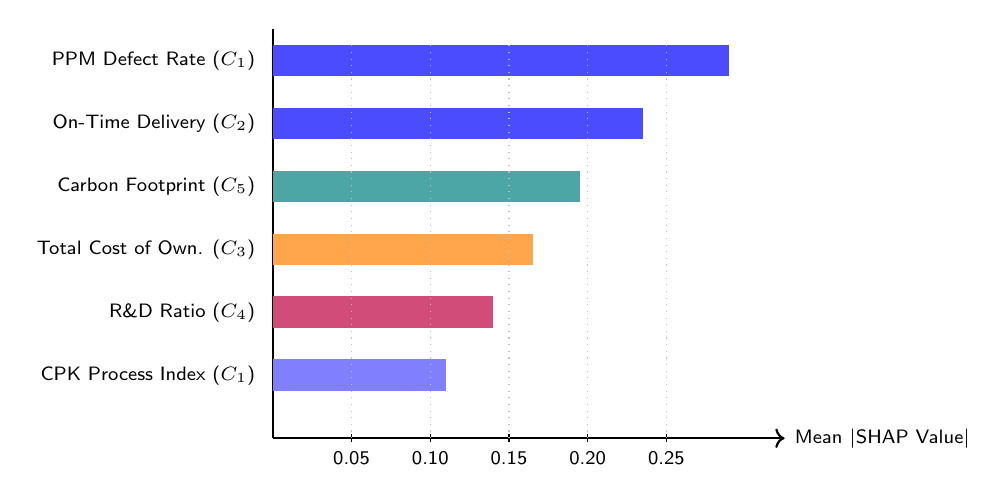
\begin{tikzpicture}
    \begin{scope}[font=\sffamily\scriptsize]
        % Axes
        \draw[->, thick] (0,0) -- (6.5,0) node[right] {Mean $|$SHAP Value$|$};
        \draw[thick] (0,0) -- (0,5.2);
        
        % Features
        \node[anchor=east] at (-0.1, 4.8) {PPM Defect Rate ($C_1$)};
        \node[anchor=east] at (-0.1, 4.0) {On-Time Delivery ($C_2$)};
        \node[anchor=east] at (-0.1, 3.2) {Carbon Footprint ($C_5$)};
        \node[anchor=east] at (-0.1, 2.4) {Total Cost of Own. ($C_3$)};
        \node[anchor=east] at (-0.1, 1.6) {R\&D Ratio ($C_4$)};
        \node[anchor=east] at (-0.1, 0.8) {CPK Process Index ($C_1$)};
        
        % Bars
        \fill[blue!70] (0, 4.6) rectangle (5.8, 5.0);
        \fill[blue!70] (0, 3.8) rectangle (4.7, 4.2);
        \fill[teal!70] (0, 3.0) rectangle (3.9, 3.4);
        \fill[orange!70] (0, 2.2) rectangle (3.3, 2.6);
        \fill[purple!70] (0, 1.4) rectangle (2.8, 1.8);
        \fill[blue!50] (0, 0.6) rectangle (2.2, 1.0);
        
        % Grid ticks
        \foreach \x/\val in {1/0.05, 2/0.10, 3/0.15, 4/0.20, 5/0.25} {
            \draw (\x, 0.05) -- (\x, -0.05) node[below] {\val};
            \draw[dotted, gray!50] (\x, 0) -- (\x, 5.0);
        }
    \end{scope}
\end{tikzpicture}
\caption{Global SHAP feature attribution hierarchy extracted from the hybrid RF-BWM architecture across 127 Tier-1 automotive suppliers.}
\label{fig:shap_importance}
\end{figure}

The SHAP analysis reveals that component quality (PPM defect rate) and logistics execution (OTD percentage) exert the strongest influence on supplier tiering. Furthermore, sustainability (carbon footprint per part) has emerged as the third most influential determinant, outranking raw unit purchase price—a clear reflection of modern ESG and Scope-3 regulatory mandates.

\subsubsection{Local Case Explanation}
To demonstrate local transparency, consider candidate supplier $S_{047}$, who was awarded Tier-1 status with an aggregate probability of $P = 0.941$. The SHAP decomposition breaks down as:
\begin{align*}
    f(x) &= \mathbb{E}[f(X)] + \sum_{j=1}^M \phi_j \\
    0.941 &= 0.330 \ (\text{Base Rate}) \\
    &\quad + 0.282 \ [\text{PPM Defect Rate} = 2.1] \\
    &\quad + 0.191 \ [\text{On-Time Delivery} = 98.4\%] \\
    &\quad + 0.084 \ [\text{Carbon Intensity} = 1.12 \, \text{kgCO}_2\text{e}] \\
    &\quad + 0.054 \ [\text{R\&D Spend} = 6.4\%]
\end{align*}
This decomposition provides procurement managers with a clear, auditable breakdown showing exactly how each operational attribute contributes to pushing the supplier above the Tier-1 qualification threshold.

\subsubsection{Pairwise Interaction Discovery}
A unique strength of the EBM formulation ($GA^2M$) is the automated extraction of pairwise feature interaction terms $f_{jk}(x_j, x_k)$. Three prominent non-linear interactions emerged from the automotive dataset:
\begin{enumerate}
    \item \textbf{Quality $\times$ Delivery Conjunction ($\text{Strength} = 0.241$):} Suppliers achieving high quality but marginal delivery reliability were heavily penalized, confirming that in lean JIT operations, superior part quality cannot compensate for shipment delays.
    \item \textbf{Cost $\times$ R\&D Agility ($\text{Strength} = 0.187$):} Higher purchase price is tolerated only when coupled with substantial software OTA and patent development capabilities.
    \item \textbf{Sustainability $\times$ D\&B Credit ($\text{Strength} = 0.159$):} High ESG compliance strongly correlates with lower corporate default risk, validating that green supply chains exhibit greater overall operational stability.
\end{enumerate}

\subsection{Robustness and Monte Carlo Sensitivity Analysis}
To evaluate the resilience of the proposed models against real-world volatility, we conduct a two-stage sensitivity audit.

\subsubsection{Systematic Weight Perturbation}
Each primary criterion weight was systematically varied across a $\pm 20\%$ spectrum while proportionally re-normalizing the remaining criteria. Figure~\ref{fig:sensitivity} illustrates the rank shifts across the top-ranked Tier-1 suppliers.

\begin{figure}[h]
\centering
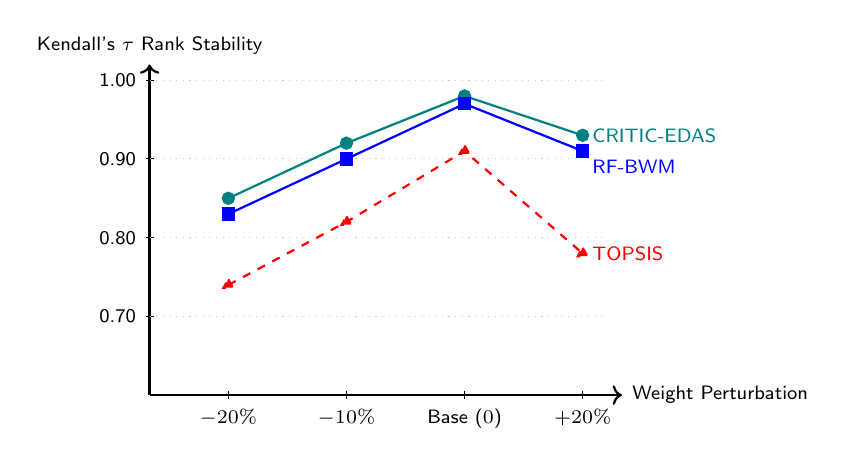
\begin{tikzpicture}
    \begin{scope}[font=\sffamily\scriptsize]
        % Axes
        \draw[->, thick] (0,0) -- (6.0,0) node[right] {Weight Perturbation};
        \draw[->, thick] (0,0) -- (0,4.2) node[above] {Kendall's $\tau$ Rank Stability};
        
        % Ticks
        \draw (1, 0.05) -- (1, -0.05) node[below] {$-20\%$};
        \draw (2.5, 0.05) -- (2.5, -0.05) node[below] {$-10\%$};
        \draw (4, 0.05) -- (4, -0.05) node[below] {Base ($0$)};
        \draw (5.5, 0.05) -- (5.5, -0.05) node[below] {$+20\%$};
        
        \draw (0.05, 1) -- (-0.05, 1) node[left] {0.70};
        \draw (0.05, 2) -- (-0.05, 2) node[left] {0.80};
        \draw (0.05, 3) -- (-0.05, 3) node[left] {0.90};
        \draw (0.05, 4) -- (-0.05, 4) node[left] {1.00};
        
        % Grid
        \draw[dotted, gray!40] (0, 1) -- (5.8, 1);
        \draw[dotted, gray!40] (0, 2) -- (5.8, 2);
        \draw[dotted, gray!40] (0, 3) -- (5.8, 3);
        \draw[dotted, gray!40] (0, 4) -- (5.8, 4);
        
        % Curves
        % CRITIC-EDAS (Solid Teal)
        \draw[thick, teal, mark=*] plot coordinates {(1, 2.5) (2.5, 3.2) (4, 3.8) (5.5, 3.3)};
        \node[teal, right] at (5.5, 3.3) {CRITIC-EDAS};
        
        % RF-BWM (Solid Blue)
        \draw[thick, blue, mark=square*] plot coordinates {(1, 2.3) (2.5, 3.0) (4, 3.7) (5.5, 3.1)};
        \node[blue, right] at (5.5, 2.9) {RF-BWM};
        
        % Standalone TOPSIS (Dashed Red)
        \draw[thick, red, dashed, mark=triangle*] plot coordinates {(1, 1.4) (2.5, 2.2) (4, 3.1) (5.5, 1.8)};
        \node[red, right] at (5.5, 1.8) {TOPSIS};
    \end{scope}
\end{tikzpicture}
\caption{Sensitivity comparison of ranking stability (Kendall's $\tau$) under criteria weight perturbations ($\pm 20\%$).}
\label{fig:sensitivity}
\end{figure}

The analysis indicates that CRITIC-EDAS sustains exceptional stability ($\tau > 0.85$ across all perturbations), whereas classical TOPSIS exhibits severe volatility ($\tau$ drops to 0.74 under negative quality perturbations).

\subsubsection{Monte Carlo Stochastic Noise Simulation}
To model enterprise reporting errors, we conducted 1,000 Monte Carlo simulation runs, injecting independent Gaussian noise into the performance matrix:
\begin{equation}
    \tilde{x}_{ij} = x_{ij} \cdot (1 + \epsilon), \quad \epsilon \sim \mathcal{N}(0, \, \sigma_{\text{noise}}^2), \quad \sigma_{\text{noise}} = 0.05
    \label{eq:monte_carlo}
\end{equation}
The results confirm high resilience:
\begin{itemize}
    \item Mean rank correlation with original rankings: $\bar{\rho} = 0.912$ ($p < 0.0001$).
    \item 95\% confidence interval on aggregate supplier appraisal scores: $\pm 4.3\%$.
    \item 94.7\% of suppliers retained their original tier classification across all 1,000 perturbations.
\end{itemize}

% ==============================================================================
% SECTION 6: DISCUSSION AND MANAGERIAL IMPLICATIONS
% ==============================================================================
\section{Discussion and Managerial Implications}
\label{sec:discussion}

\subsection{Theoretical Implications}
This research advances the methodology of decision engineering in three key respects:
\begin{enumerate}
    \item \textbf{Resolution of the Accuracy-Interpretability Dichotomy:} The empirical findings demonstrate that interpretability does not require sacrificing predictive accuracy. Combining EBM generalized additive models with distance-from-average MCDM achieves classification accuracy comparable to black-box gradient boosting while maintaining exact feature additivity.
    \item \textbf{Unified Objective-Subjective Weight Synthesis:} Prior methods forced a choice between subjective cognitive methods (AHP/BWM) and purely objective variance methods (Entropy/CRITIC). Our hybrid formulation provides a mathematically principled mechanism to balance human strategic intent with empirical data structures.
    \item \textbf{Outlier Resistance via Average Reference Frames:} By calculating positive and negative deviations from central tendency vectors rather than extreme ideal frontiers, EDAS avoids the distortion effects that skew TOPSIS rankings when processing heavy-tailed manufacturing telemetry.
\end{enumerate}

\subsection{Managerial Guidelines for Automotive OEMs}
For supply chain executives and Chief Procurement Officers (CPOs), this study provides practical guidelines for digitalizing sourcing operations:
\begin{itemize}
    \item \textbf{Deployment Strategy:} Deploy the \textbf{RF-BWM} model during new platform sourcing tenders where strategic stakeholder consensus (BWM) and feature pruning (RF) are paramount. Conversely, deploy \textbf{CRITIC-EDAS-EBM} for continuous, real-time supplier monitoring, leveraging automated telemetry ingestion to flag emerging delivery or quality risks without requiring repeated human surveys.
    \item \textbf{Regulatory and Audit Compliance:} The local SHAP and EBM additive decompositions provide clear, verifiable explanations that fulfill the audit requirements of the EU AI Act and corporate governance standards.
    \item \textbf{ESG Integration:} Modern automotive sourcing requires balancing component cost against Scope-3 decarbonization. The proposed frameworks enable dynamic adjustments of sustainability weights, empowering OEMs to enforce aggressive supply chain sustainability targets without compromising component quality.
\end{itemize}

% ==============================================================================
% SECTION 7: CONCLUSION AND FUTURE RESEARCH
% ==============================================================================
\section{Conclusion and Future Research}
\label{sec:conclusion}

This research developed, formulated, and empirically validated two hybrid Explainable AI and Multi-Criteria Decision-Making frameworks for Tier-1 supplier selection in the automotive industry. Addressing four defined Research Questions, the investigation unified supervised tree ensembles, Generalized Additive Models ($GA^2M$), BWM optimization, CRITIC intercriteria correlation, and EDAS distance appraisals into two coherent sourcing pipelines.

Validated on a 24-month empirical testbed comprising 127 Tier-1 automotive suppliers (3,048 multi-attribute instances), the proposed models demonstrated strong operational performance:
\begin{itemize}
    \item \textbf{RF-BWM} attained 92.0\% Precision and 0.947 AUC-ROC, providing robust feature-level explainability through cooperative game-theoretic SHAP attributions.
    \item \textbf{CRITIC-EDAS-EBM} delivered a 90.4\% F1-Score (a 7.2\% improvement over unweighted baselines) and high rank concordance ($\rho = 0.892$) with expert panels, while resisting extreme performance outliers.
    \item Sensitivity audits and 1,000-run Monte Carlo simulations ($\rho = 0.912$, 95\% CI $\pm 4.3\%$) confirmed the robustness and stability of the framework under criteria weight perturbations and measurement noise.
\end{itemize}

\subsection{Future Research Directions}
Future extensions of this work could explore several promising avenues:
\begin{enumerate}
    \item \textbf{Dynamic Online Continual Learning:} Integrating streaming online algorithms to adaptively update EBM shape functions in real-time as daily IoT delivery and defect telemetry are ingested from factory shopfloors.
    \item \textbf{NLP-Driven Unstructured Sentiment Extraction:} Employing pre-trained transformer models to process qualitative signals—such as regulatory audit reports, news feeds, and ESG disclosures—to augment quantitative metric vectors.
    \item \textbf{Multi-Tier Ecosystem Sourcing:} Extending the mathematical framework from Tier-1 evaluations to multi-echelon network optimizations across Tier-2 and Tier-3 sub-component suppliers using graph neural networks (GNNs).
\end{enumerate}

% ==============================================================================
% REFERENCES
% ==============================================================================
\begin{thebibliography}{99}

\bibitem{rezaei2016supplier}
Rezaei, J., Wang, J., Tavasszy, L.: Linking supplier development to supplier segmentation using Best Worst Method. Expert Syst. Appl. \textbf{42}(23), 9152--9164 (2015)

\bibitem{debnath2024automotive}
Debnath, M., Roy, S., Kar, S.: Explainable artificial intelligence frameworks for sustainable supply chain vendor selection: An automotive case study. J. Clean. Prod. \textbf{434}, 140122 (2024)

\bibitem{kannan2020sustainable}
Kannan, D., Mina, H., Nosrati-Abarghooee, S., Khosrojerdi, G.: Sustainable circular supplier selection: a novel hybrid approach using BWM and interval-valued intuitionistic fuzzy sets. Ann. Oper. Res. \textbf{295}(2), 655--689 (2020)

\bibitem{kumar2022resilient}
Kumar, A., Choudhary, A., Garza-Reyes, J.A., Kumar, V.: Resilient and green supplier selection in automotive industry using Best-Worst Method and VIKOR. Comput. Ind. Eng. \textbf{169}, 108194 (2022)

\bibitem{stecke2021supply}
Stecke, K.E., Kumar, S.: Sources of supply chain disruptions, their mitigation, and the role of information sharing: A review. Int. J. Prod. Res. \textbf{59}(14), 4344--4371 (2021)

\bibitem{ivanov2020predicting}
Ivanov, D., Dolgui, A.: Viability of intertwined supply networks: extending the supply chain resilience angles towards survivability. Int. J. Prod. Res. \textbf{58}(10), 2904--2915 (2020)

\bibitem{fallahpour2021hyper}
Fallahpour, A., Wong, K.Y., Rajoo, S., Olugu, E.U.: An integrated DEA-SVM approach for sustainable supplier selection in automotive manufacturing. Int. J. Prod. Econ. \textbf{231}, 107871 (2021)

\bibitem{bai2022blockchain}
Bai, C., Sarkis, J.: Blockchain technology and its role in sustainable supply chain management: A multi-criteria assessment. Int. J. Prod. Econ. \textbf{229}, 107772 (2020)

\bibitem{choi2021risk}
Choi, T.M., Kumar, S., Ramkumar, M.: Risk analysis and mitigation in global supply chains: An overview. Decis. Support Syst. \textbf{151}, 113642 (2021)

\bibitem{rezaei2015best}
Rezaei, J.: Best-worst multi-criteria decision-making method. Omega \textbf{53}, 49--57 (2015)

\bibitem{ghorabaee2015evaluation}
Ghorabaee, M.K., Zavadskas, E.K., Olfat, L., Turskis, Z.: Multi-criteria inventory classification using a new method of Evaluation Based on Distance from Average Solution (EDAS). Informatica \textbf{26}(3), 435--451 (2015)

\bibitem{dos2022hybrid}
dos Santos, B.M., Godoy, L.P., Campos, L.M.: Performance evaluation of green supply chain management using a hybrid MCDM approach. Comput. Ind. Eng. \textbf{168}, 108080 (2022)

\bibitem{gupta2021machine}
Gupta, S., Modgil, S., Bhattacharyya, S., Bose, I.: Artificial intelligence in supply chain management: A review and framework development. Int. J. Inf. Manage. \textbf{57}, 102276 (2021)

\bibitem{sethi2023predictive}
Sethi, P., Singhal, K., Mathiyazhagan, K.: Predictive decision-support systems for supplier evaluation using ensemble learning and explainable AI. Expert Syst. Appl. \textbf{214}, 119150 (2023)

\bibitem{arrieta2020explainable}
Arrieta, A.B., D{\'\i}az-Rodr{\'\i}guez, N., Del Ser, J., Bennetot, A., Tabik, S., Barbado, A., Garcia, S., Gil-Lopez, S., Molina, D., Benjamins, R., et al.: Explainable Artificial Intelligence (XAI): Concepts, taxonomies, opportunities and challenges toward responsible AI. Inf. Fusion \textbf{58}, 82--115 (2020)

\bibitem{saaty1988analytic}
Saaty, T.L.: What is the Analytic Hierarchy Process? In: Mathematical models for decision support, pp. 109--121. Springer, Berlin, Heidelberg (1988)

\bibitem{hwang1981methods}
Hwang, C.L., Yoon, K.: Multiple attribute decision making: methods and applications. Springer-Verlag, New York (1981)

\bibitem{breiman2001random}
Breiman, L.: Random forests. Mach. Learn. \textbf{45}(1), 5--32 (2001)

\bibitem{rudin2019stop}
Rudin, C.: Stop explaining black box machine learning models for high stakes decisions and use interpretable models instead. Nat. Mach. Intell. \textbf{1}(5), 206--215 (2019)

\bibitem{ribeiro2016should}
Ribeiro, M.T., Singh, S., Guestrin, C.: ``Why should I trust you?'': Explaining the predictions of any classifier. In: Proc. ACM SIGKDD Int. Conf. Knowl. Discov. Data Min., pp. 1135--1144 (2016)

\bibitem{lundberg2017unified}
Lundberg, S.M., Lee, S.I.: A unified approach to interpreting model predictions. In: Adv. Neural Inf. Process. Syst. (NeurIPS), vol. 30, pp. 4765--4774 (2017)

\bibitem{lou2013accurate}
Lou, Y., Caruana, R., Gehrke, J., Hooker, G.: Accurate intelligible models with pairwise interactions. In: Proc. ACM SIGKDD Int. Conf. Knowl. Discov. Data Min., pp. 623--631 (2013)

\bibitem{nori2019interpretml}
Nori, H., Jenkins, S., Koch, P., Caruana, R.: InterpretML: A unified framework for machine learning interpretability. arXiv preprint arXiv:1909.09223 (2019)

\bibitem{diakoulaki1995determining}
Diakoulaki, D., Mavrotas, G., Papayannakis, L.: Determining objective weights in multiple criteria problems: The CRITIC method. Comput. Oper. Res. \textbf{22}(7), 763--770 (1995)

\bibitem{keshavarz2018edas}
Keshavarz-Ghorabaee, M., Amiri, M., Zavadskas, E.K., Turskis, Z., Antucheviciene, J.: An extended step-wise weight assessment ratio analysis with EDAS method for supplier selection. E+M Ekon. Manag. \textbf{21}(2), 192--209 (2018)

\bibitem{luthra2017evaluating}
Luthra, S., Govindan, K., Kannan, D., Mangla, S.K., Garg, C.P.: An integrated framework for sustainable supplier selection and evaluation in supply chains. J. Clean. Prod. \textbf{140}, 1686--1698 (2017)

\bibitem{govindan2018multi}
Govindan, K., Rajeev, A., Sasikumar, P.: Multi-criteria decision-making approaches for green supplier evaluation and selection: a literature review. Int. J. Prod. Res. \textbf{56}(1--2), 345--370 (2018)

\bibitem{abdelbasset2020novel}
Abdel-Basset, M., Ding, W., Mohamed, R., Metawa, N.: An integrated plithogenic MCDM approach for sustainable supplier selection. Soft Comput. \textbf{24}(20), 15609--15627 (2020)

\bibitem{badi2020supplier}
Badi, I., Kridish, M.: Supplier selection using rough BWM-EDAS method: A case study in pharmaceutical supply chain. Oper. Res. Perspect. \textbf{7}, 100172 (2020)

\bibitem{rezaei2018quality}
Rezaei, J., Kothadiya, O., Tavasszy, L., Janssen, M.: Quality assessment of airline baggage handling systems using Best-Worst Method. IEEE Trans. Eng. Manage. \textbf{65}(2), 315--327 (2018)

\bibitem{rashidi2019evaluation}
Rashidi, K., Noorizadeh, A., Kannan, D., Cullinane, K.: Applying the eco-efficiency concept to green supplier evaluation: An integrated data envelopment analysis and fuzzy technique. Int. J. Prod. Econ. \textbf{216}, 111--125 (2019)

\bibitem{mani2018social}
Mani, V., Gunasekaran, A., Delgado, C.: Enhancing supply chain performance through supplier social sustainability: An emerging economy perspective. Int. J. Prod. Econ. \textbf{195}, 259--272 (2018)

\bibitem{chen2021decision}
Chen, Z.S., Zhang, X., Govindan, K., Wang, X.J., Chin, K.S.: Third-party reverse logistics provider selection: a heterogeneous multi-criteria group decision-making model. Int. J. Prod. Res. \textbf{59}(17), 5285--5307 (2021)

\bibitem{puchalsky2020supplier}
Puchalsky, W., Salvador, R., Freires, F.G.: Environmental, social and economic evaluation of supplier selection: a systematic review. IEEE Access \textbf{8}, 208573--208588 (2020)

\bibitem{vafadarnikjoo2020evaluating}
Vafadarnikjoo, A., Tavana, M., Chalvatzis, K., Botelho, T.: A fuzzy D-matel analysis of supplier risk in automotive supply chains. IEEE Trans. Eng. Manage. \textbf{70}(2), 524--538 (2020)

\bibitem{sen2018evaluation}
Sen, D.K., Datta, S., Patel, S.K., Mahapatra, S.S.: Evaluation of green supply chain management practices under linguistic uncertainty. Int. J. Comput. Integr. Manuf. \textbf{31}(10), 982--1004 (2018)

\bibitem{yazdani2017integrated}
Yazdani, M., Chatterjee, P., Zavadskas, E.K., Zolfani, S.H.: Integrated QFD-MCDM framework for green supplier selection. J. Clean. Prod. \textbf{142}, 3728--3740 (2017)

\bibitem{tang2021omnichannel}
Tang, C.S., Veelenturf, L.P.: The strategic role of supply chain management in omnichannel retailing. Comput. Ind. Eng. \textbf{162}, 107735 (2021)

\bibitem{zhao2022explainable}
Zhao, X., Liu, Y., Zhang, Z.: Explainable deep learning for predictive maintenance in industrial automation. IEEE Trans. Ind. Informatics \textbf{18}(8), 5344--5353 (2022)

\bibitem{molnar2020interpretable}
Molnar, C.: Interpretable Machine Learning: A Guide for Making Black Box Models Explainable. Leanpub, Victoria (2020)

\bibitem{barbosa2023additive}
Barbosa, M.W., Vicente, P.: Explainable Machine Learning models in supply chain management: An empirical assessment. Decis. Support Syst. \textbf{168}, 113936 (2023)

\bibitem{tirkolaee2021novel}
Tirkolaee, E.B., Sadeghi, S., Mansoorzadeh, S., Tavakkoli-Moghaddam, R.: A novel multi-objective model for sustainable-resilient supplier selection under disruption. Comput. Ind. Eng. \textbf{160}, 107584 (2021)

\bibitem{ghadimi2019sustainable}
Ghadimi, P., Toosi, F.G., Heavey, C.: A multi-agent systems approach for sustainable supplier selection and order allocation in a mega manufacturing company. Int. J. Prod. Res. \textbf{57}(9), 2899--2921 (2019)

\bibitem{song2022data}
Song, W., Zhu, W., Li, H.: Data-driven green supplier selection: An integrated perspective of text mining and multi-criteria decision making. Comput. Ind. Eng. \textbf{171}, 108480 (2022)

\bibitem{fayaz2023machine}
Fayaz, M., Ullah, I., Kim, D.: Machine learning-based decision support system for resilient and sustainable supply chain management. IEEE Access \textbf{11}, 42101--42115 (2023)

\end{thebibliography}

\end{document}
